\documentclass[12pt,a4paper,twoside]{book}

%%%%%%%%%%%%%%%%%%%%%%%%%%%%%%%%%%%%%%%%%%%%%%%%%%%%%%%%%%%%%%%%%%%%%%%%
%%%%%%%%%%%% Packages %%%%%%%%%%%%%%%%%%%%%%%%%%%%%%%%%%%%%%%%%%%%%%%%%%
%%%%%%%%%%%%%%%%%%%%%%%%%%%%%%%%%%%%%%%%%%%%%%%%%%%%%%%%%%%%%%%%%%%%%%%%

%%%%%%
% In general useful packages
%%%%%%
\usepackage[latin1]{inputenc} % allow Umlauts
\usepackage[T1]{fontenc} % Umlauts as character in font
\usepackage{fancyhdr}   % Header/Footer
\usepackage[pdftex]{graphicx}
\usepackage{amsmath, amsthm, amssymb, amsfonts}

%%%%%%
% The following packages are optional, uncomment them if useful and required
%%%%%%
\usepackage{fancyvrb}   % extended verbatim environment
% \usepackage{latexsym}   % additional symbols
% \usepackage{times}      % bessere Schrift in PS-Dateien
% \usepackage{longtable}  % long tables (with page breaks)
% \usepackage{breakcites}  % linebreaks in cites

\usepackage[us]{datetime} % date in \today as "Month DD, YYYY", e.g., "February 29, 2012"


%%%%%%
% Hyperlinks in PDF output (blue borders, text color unchanged)
%%%%%%
\usepackage[plainpages=false, pdfpagelabels, bookmarks,  colorlinks=false,
               linkbordercolor={0 0 1}, filebordercolor={0 0 1}, citebordercolor={0 0 1},
               menubordercolor={0 0 1}, urlbordercolor={0 0 1}]{hyperref}

%%%%%%
% Another set of useful packages
%%%%%%
% \usepackage[square]{natbib}  % more powerful and customizable references
% \usepackage[center]{caption} % centered, multi-line captions of figures and tables
% \usepackage{floatflt}        % floats (e.g., figures & tables) which can have floating text around them
% \usepackage[thmmarks]{ntheorem}    % extended theorem environment
\usepackage{pdfcomment}  % comments in text as PDF notes

%%%%%%%%%%%%%%%%%%%%%%%%%%%%%%%%%%%%%%%%%%%%%%%%%%%%%%%%%%%%%%%%%%%%%%%%
%%%%%%%%%%%% Layout %%%%%%%%%%%%%%%%%%%%%%%%%%%%%%%%%%%%%%%%%%%%%%%%%%
%%%%%%%%%%%%%%%%%%%%%%%%%%%%%%%%%%%%%%%%%%%%%%%%%%%%%%%%%%%%%%%%%%%%%%%%
% German style (no paragraph indent, but gap between paragraphs)
 \setlength{\parindent}{0mm}
% \setlength{\parskip}{4pt plus3pt minus2pt}

% Page width and margins (usually no need to change, just use a4wide package)
% \setlength{\textwidth}{15cm}
% \addtolength{\oddsidemargin}{1mm}
% \addtolength{\evensidemargin}{-13.5mm}
\usepackage{a4wide} % better than individual setup

% For fancyhdr, otherwise it might result in "overfull vbox"
\addtolength{\headheight}{3.5pt}

% URL Prefix for Bibliography (i.e., no prefix, typewriter as font for URLs)
\newcommand{\urlprefix}{}
\def\UrlFont{\small\tt}
%\urlstyle{rm} % oder sf, falls obiges nicht funktioniert


%%%%%%%%%%%%%%%%%%%%%%%%%%%%%%%%%%%%%%%%%%%%%%%%%%%%%%%%%%%%%%%%%%%%%%%%
%%%%%%%%%%%% Some useful macros %%%%%%%%%%%%%%%%%%%%%%%%%%%%%%%%%%%%%%%%
%%%%%%%%%%%%%%%%%%%%%%%%%%%%%%%%%%%%%%%%%%%%%%%%%%%%%%%%%%%%%%%%%%%%%%%%

% myfigure: filename width caption
\newcommand{\myfigure}[3]{%
  \begin{figure}
    \centerline{\includegraphics[width=#2]{figures/#1.pdf}}
  \caption{#3}
  \label{fig:#1}
  \end{figure}
}

% Floating figures = figures with floating text around: filename width caption
\newcommand{\myfloatfigure}[3]{%
  \begin{floatingfigure}{#2}
    \includegraphics[width=#2]{figures/#1.pdf}
  \caption{#3}
  \label{fig:#1}
  \end{floatingfigure}
}

% two figures side by side: file1 width1 caption1 file2 width2 caption2
\newcommand{\mydoublefigure}[6]{%
  \begin{figure}
  \begin{minipage}[t]{#2}
    \centerline{\includegraphics[width=\textwidth]{figures/#1.pdf}}
  \centering
  \caption{#3}
  \label{fig:#1}
  \end{minipage}
  \hfill
  \begin{minipage}[t]{#5}
    \centerline{\includegraphics[width=\textwidth]{figures/#4.pdf}}
  \centering
  \caption{#6}
  \label{fig:#4}
  \end{minipage}
  \end{figure}
}


% Better verbatim environments (requires fancyvrb package)
\DefineVerbatimEnvironment{myverb}{Verbatim}{fontsize=\small,baselinestretch=0.84}
\DefineVerbatimEnvironment{myverbbox}{Verbatim}{frame=single,fontsize=\small,baselinestretch=0.84}


% For figures and tables
\renewcommand{\topfraction}{0.9} % a page has at most 90% of floats and at least 10% of text (if page contains floats AND text)
\renewcommand{\bottomfraction}{0.9}
\renewcommand{\floatpagefraction}{0.7} % a page with floats only is at least 70% full

% Hyphenation (include a special file with hyphenation hints if there are problems)
% \include{myhyphen}



\begin{document}

\iffalse
% Title page
\begingroup
  \pagenumbering{roman}
  \include{title}

\newpage

\thispagestyle{empty}

\rule{0cm}{5cm}

\newpage

\thispagestyle{empty}

\include{declaration}

%%% Include abstract and acknowledgements as necessary
\include{acknowledgements}
\include{abstract}

\newpage

\endgroup

%%%%%%%%%%%%%%%%%%%
% Header & footers
%%%%%%%%%%%%%%%%%%%

\pagestyle{fancy}

% Headers with page numbers and section/chapter titles
\renewcommand{\sectionmark}[1]{\markright{\thesection\ #1}}
\renewcommand{\chaptermark}[1]{\markboth{\thechapter\ #1}{}}
\lhead[\rm\thepage]{\sl\rightmark}
\chead{}
\rhead[\sl\leftmark]{\rm\thepage}

% Footers empty
\lfoot{}
\cfoot{}
\rfoot{}


\tableofcontents

% Include also list of figures and tables if useful
%\listoffigures
%\listoftables

\fi

%%%%%%%%%%%%%%%%%%%%
%%% Contents %%%%%%%
%%%%%%%%%%%%%%%%%%%%
% Put each chapter in a separate file

\chapter{Introduction}
\label{cha:intro}

% Important: you have to switch to arabic numbering here!
\pagenumbering{arabic}


\section{Distributed word representations}


\section{Polysemy}

\section{Thesis Organization}

\chapter{Knowledge}
\label{cha:knowledgei}

\section{Prerequisites}
This section will introduce some important knowledges, including sigmoid function, Bayes Formula, Huffman code, etc.

\subsection{Sigmoid Function}
Sigmoid function is a common kind of active function, the definition is
$$ \sigma(x) = \frac{1}{1+e^{-x}}, $$
The domain is $(-\infty, \infty)$, the range is $(0,1)$. And Figure~\ref{fig:sigmoid} shows the sigmoid function.
\begin{figure}[!ht]
  \centering
	\fbox{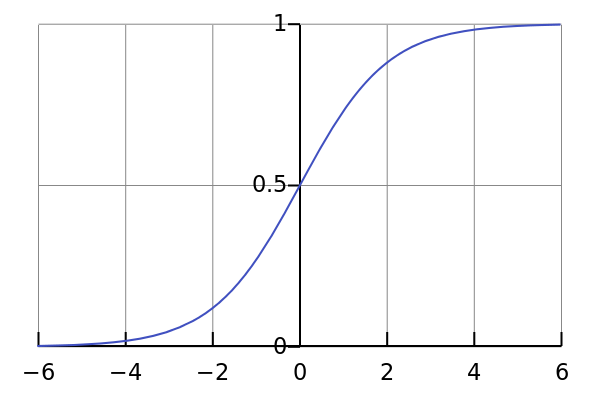
\includegraphics[width=0.5\textwidth]{sigmoid} }
	\caption{Sigmoid Function}
	\label{fig:sigmoid}
\end{figure}

Sigmoid function has the \textbf{derivative function} as following:
$$ \sigma^\prime(x) = \sigma(x)[1-\sigma(x)], $$
Thus, the \textbf{derivative functions} of $\mathrm{log}\sigma(x)$ and $\mathrm{log}(1-\sigma(x))$ are respectively
\begin{equation} 
[\mathrm{log}\sigma(x)]^\prime = 1-\sigma(x), \ [\mathrm{log}(1-\sigma(x))]^\prime = -\sigma(x), 
\end{equation}
Equation (2.1) will be used later in the derivation.

\subsection{Logistic Regression}
Binary classification is a very common task, e.g. , if an email is spam, if a customer is a potential customer, if a online transaction fraud, etc. Let ${\{(\mathbf{x}_i,y_i)\}}^m_{i=1}$ be the sample data of a binary classification problem, where $\mathbf{x}_i \in \mathbb{R}^n$, $y_i \in \{0,1\}$, when $y_i = 1$ the corresponding sample is $\mathbf{positive}$, when $y_i = 0$ the corresponding sample is $\mathbf{negative}$.

As for some sample data $\mathbf{x} = (x_1,x_2,\cdots,x_n)^T$, the hypothesis function can be written as
$$h_\theta(\mathbf{x}) = \sigma(\theta_0+\theta_1 x_1+\theta_2 x_2+\cdots+\theta_n x_n),$$
where $\theta = (\theta_0,\theta_1,\cdots,\theta_n)^T$ is the undetermined parameter. To simplify the formula, introduce $x_0 = 1$, and then $\mathbf{x}$ is extended to $(x_0,x_1,x_2,\cdots,x_n)^T$. Without confusing it is also recorded as $\mathbf{x}$. Thus, $h_0$ can be simplified as 
$$h_\theta(\mathbf{x}) = \sigma(\theta^T \mathbf{x}) = \frac{1}{1+e^{-\theta^T \mathbf{x}}}.$$

Let threshold $T = 0.5$, then the discriminant formula for binary classification is
$$y(\mathbf{x})=
\begin{cases}
1,& h_\theta(\mathbf{x})\geq 0.5;\\
0,& h_\theta(\mathbf{x})\le 0.5.
\end{cases}$$

How to calculate $\theta$ ? The usual method is, firstly determine a form of the \textbf{overall loss function} as following
$$ J(\theta) = \frac{1}{m}\sum^m_{i=1}cost(\mathbf{x}_i,y_i),$$
and then optimize it to obtain the optimal parameters $\theta^*$.

In practice, the loss function of a single sample $cost(\mathbf{x}_i,y_i)$ is often taken as the \textbf{log-likelihood function}
$$cost(\mathbf{x}_i,y_i)=
\begin{cases}
-\mathrm{log}(h_\theta(\mathbf{x}_i)),& y_i=1;\\
-\mathrm{log}(1-h_\theta(\mathbf{x}_i)),& y_i=0.
\end{cases}$$
Note that the above formula is a piecewise function, which can also be written in its overall expression as following
$$cost(\mathbf{x}_i,y_i) = -y_i\cdot\mathrm{log}(h_\theta(\mathbf{x}_i))-(1-y_i)\cdot(1-h_\theta(\mathbf{x}_i)).$$

\subsection{Bayes Formula}
Bayesian formula is put forward by the British mathematician Thomas Bayes, used to describe the relationship between two conditional probabilities. Let $P(A)$ and $P(B)$ respectively be the probability of event A and the probability of event B, $P(A|B)$ be the probability of the event A when event B occurs, and $P(A,B)$ be the probability of event A and B occurring simultaneously, so we have
$$P(A|B)=\frac{P(A,B)}{P(B)}, P(B|A)=\frac{P(A,B)}{P(A)}, $$
further, we can get
$$P(A|B)=P(A)\frac{P(B|A)}{P(B)},$$
this is the \textbf{Bayesian formula}.

\subsection{Huffman Coding}

\subsubsection{Huffman Tree}
In computer science, \textbf{tree} is a kind of nonlinear data structure, which is the structure of data elements (called \textbf{node} in the tree) organized in branch. The collection of several disjoint trees is called \textbf{forest}. The following are some common concepts about tree.
\begin{itemize}
\item \textbf{Path} and \textbf{Path Length}\\
In a tree, a path is a road from any node to its direct or indirect child. The number of branches is called path length of the path. If the provisions of the root layer No. 1, from the root node to the first node L layer path length L-1.
\item \textbf{Weighted Node} and \textbf{Weighted Path Length}\\
blabla..
\end{itemize}

\subsubsection{Huffman Tree Construction}

\subsubsection{Huffman Coding}

%--------------------------------------------------------------------------------------------------------------------------------%

\section{Skip-gram model}




\chapter{Word Embedding}
\label{cha:embedi}

\section{Introduction}

\subsection{Word2vec and distributional semantics}
Word2vec is closely related to earlier (non-neural-net) approaches\\

Don\rq t count, predict! A systematic comparison of context-counting vs. context-predicting semantic vectors (Baroni et al, 2014)\\

Word2vec found better on average \& more robust than DS techniques (Baroni et al, 2014\\

Neural word embedding as implicit matrix factoriza5on (Levy \& Goldberg, 2014) \\

Glove: Global Vectors for Word Representa5on (Pennington et al, 2014)\\

Main findings: the word2vec \lq\lq trick\rq\rq can be ported back to the traditional DS techniques\\

\subsection{And some controversy}
Glove: Global Vectors for Word Representa5on (Pennington et al, 2014)\\

Richard Socher: \lq\lq Glove 11\% better on word analogies than ord2vec!!!\rq\rq\\

Goldberg: \lq\lq at least train the models on the same data \ldots\rq\rq\\
\\

In the end, Glove performs usually slightly worse than word2vec when both are well-tuned, and word2vec is faster \& way more memory efficient: Improving distributional similarity with lessons learned from word embeddings (Levy et al, 2015) 

\subsection{Distributed sparse representations}
Word2vec: translates 1-of-N representations into D-dimensional continuous vectors\\

The continuous vectors can be translated back into sparse vectors again, efficiently forming M-of-N codes: can be useful in time-critical applications\\

Can be achieved with random projections + quantization or max() function\\


%--------------------------------------------------------------------------------------------------------------------------------%

\section{Skip-gram model}


\textbf{Objective function:}\\

Giving a sequence of training words $w_1,w_2,w_3,\ldots,w_T$, the objective of the Skip-gram model is to maximize the average log probability 

$$\mathrm{G}=\frac{1}{T}\sum_{t=1}^T\sum_{-c\leq j\leq c,j\neq0}\mathrm{log}\ p(w_{t+j}|w_t)$$ 

where $c$ is the size of the training context. \\

\subsection{Softmax function}

The basic Skip-gram formulation defines $p(w_{t+j}|w_t)$ using the softmax function 

$$p(w_O|w_I)=\frac{\mathrm{exp}({U_{w_O}}^{\rm T}V_{w_I})}{\sum_{w=1}^W\mathrm{exp}({U_{w_O}}^{\rm T}V_{w_I})}$$ 

where $V_w$ and $U_w$ are the \lq\lq input\rq\rq\ and \lq\lq output\rq\rq\ vector representations of $w$, and $W$ is the number of words in the vocabulary.
$\nabla\mathrm{log}\ p(w_O|w_I)$ is proportional to $W$, which is often large ($10^5-10^7$ terms).\\

\subsection{Hierarchical Softmax}

It is needed to evaluate only about $\mathrm{log}_2(W)$ nodes.\\

Let $n(w,j)$ be the $j$-th node on the path from the root to $w$, and let $L(w)$ be the length of this path, so $n(w,1)$ = $\mathrm{root}$ and $n(w,L(w)) = w$. In addition, for any inner node $n$, let $ch(n)$ be an arbitrary fixed child of $n$ and let $[x]$ be $1$ if $x$ is true and $-1$ otherwise. Then the hierarchical softmax defines $p(w_O|w_I)$ as follows:

$$p(w_O|w_I)=\prod_{j=1}^{L(w)-1}\sigma\left(\left[n(w_O,j+1)=ch(n(w_O,j))\right]\cdot {U_{n(w_O,j)}}^{\rm T}V_{w_I}\right)$$

where $\sigma(x) = 1/(1+\mathrm{exp}(-x))$. It can be verified that $\sum_{w=1}^W p(w|w_I)=1$. This implies that that cost of computing $\mathrm{log}\ p(w_O|w_I)$ and $\nabla\mathrm{log}\ p(w_O|w_I)$ is proportional to $L(w_O)$, which on average is no greater than $\mathrm{log}\ W$.

\subsection{Negative Sampling}

An alternative to the hierarchical softmax is Noise Contrastive Estimation (NCE). NCE can be shown to approximately maximize the log probability of the softmax. We define Negative sampling (NEG) by the objective

$$p(w_O|w_I)=\mathrm{log}\ \sigma({U_{w_O}}^{\rm T}V_{w_I})+\sum_{i=1}^k\mathbb{E}_{w_i\sim P_n(w_O)}\left[\mathrm{log}\ \sigma(-{U_{w_i}}^{\rm T}V_{w_I})\right]$$

which is used to replace every $\mathrm{log}\ P(w_O|w_I)$ term in the Skip-gram objective. Thus the task is to distinguish the target word $w_O$ from the noise distribution $P_n(w)$ using logistic regression, where there are $k$ negative samples for each data sample. Values of $k$ in the range 5-20 are useful for small training datasets, while for large datasets the $k$ can be as small as 2-5.\\

The main difference between the Negative sampling and NCE is that NCE needs both samples and the numerical probabilities of the noise distribution, while Negative sampling uses only samples.\\

Both NCE and NEG have the noise distribution $P_n(w)$ as a free parameter.



\chapter{Models}
\label{cha:modeli}

All sense embedding models are based on the Skip-gram model. So firstly I will introduce the Skip-gram model, and then describe how other models extend the it. \\

%--------------------------------------------------------------------------------------------------------------------------------%

\section{Context clustering}


\section{Expectation-maximization algorithm}

Each Input embedding has multiple prototypes. Each prototype has a prior probability. Other things are same as skip-gram model. \\

\subsection{Some criticism for context clustering}
The performance of these multi-prototype models is quite sensitive to the clustering algorithm and requires much effort in clustering implementation and parameter tuning.\\

The lack of probabilistic explanation also refrains clustering based methods from being applied to many text mining tasks, such as language modelling. 


\subsection{Multi-Prototype Skip-Gram Model}

\textbf{Objective function:}\\
$$\mathrm{G}=\frac{1}{T}\sum_{t=1}^T\sum_{-c\leq j\leq c,j\neq0}\mathrm{log}\ p(w_{t+j}|w_t)$$ 

\textbf{Multi-Prototype Input Embedding:}\\
$$p(w_O|w_I) = \sum_{i = 1}^{N_{w_I}}P(w_O|h_{w_I}=i,w_I)P(h_{w_I}=i|w_I)$$

\textbf{Using Hierarchical Softmax:}\\
$$P(w_O|h_{w_I}=i,w_I) = \prod_{j=1}^{L(w)-1}\sigma\left(\left[n(w_O,j+1)=ch(n(w_O,j))\right]\cdot {U_{n(w_O,j)}}^{\rm T}V_{w_I,i}\right)$$ 

\subsection{EM Algorithm}

Suppose there are $M$ word pairs for training: $\{(w_1,w),(w_2,w),(w_3,w),\ldots,(w_M,w)\}$

$$\mathrm{log}\ P(\mathbb{X},$$

\textbf{E-Step:}\\

\textbf{M-Step:}\\

%--------------------------------------------------------------------------------------------------------------------------------%

\section{Sense Assignment Model (my model)}

Last model considers that only input embedding has multi-prototype. In contrast, my model considers that both input embedding and output embedding has multi-prototype. In other words, each word in sentence have different information. \\

Each iteration, fetch a batch of data. Assign sentence, update 

\subsection{Model}

\subsection{Training}

\textbf{Assignment:}\\



\textbf{}

\textbf{Train:}\\


\chapter{Implementation}
\label{cha:impl}




%\chapter{Introduction}
\label{cha:intro}

% Important: you have to switch to arabic numbering here!
\pagenumbering{arabic}


\section{Distributed word representations}


\section{Polysemy}

\section{Thesis Organization}

%\input{relwork}

%\input{solution}

%\chapter{Implementation}
\label{cha:impl}




%\input{eval}

%\input{concl}

%%% Use appendix if necessary
% \begin{appendix}
% \input{appendix}
% \end{appendix}

% References
%\input{biblio}


\end{document}


